\section{Algoritmo di Karger}
\label{cap:algorithm-karger}

\subsection{Definizione}
\label{sub:karger-definition}

\textbf{KargerMinCut} è l'implementazione dell'algoritmo randomizzato per la risoluzione del problema minimum-cut visto a lezione. L'algoritmo è di tipo \textit{Monte Carlo} e prevede i seguenti step:

\begin{enumerate}
    \item \textbf{Step 1}: La variabile \codeinline{min\_cut} viene inizializzata a $+\infty$;
    \item \textbf{Step 2}: Per $k$ iterazioni, viene eseguita la funzione \codeinline{full\_contraction};
    \item \textbf{Step 3}: Se il numero di lati del grafo ritornato da \codeinline{full\_contraction} è minore di \codeinline{min\_cut}, allora \codeinline{min\_cut} viene aggiornato a tale valore;
    \item \textbf{Step 4}: L'operazione viene ripetuta finché il grafo contiene solo 2 nodi.
\end{enumerate}

La funzione \codeinline{full\_contraction} prende in input un grafo connesso, non diretto, non pesato, ed è definita come segue:

\begin{enumerate}
    \item \textbf{Step a}: Viene creata una copia del grafo di input;
    \item \textbf{Step b}: Fino a che il grafo non contiene solo 2 nodi, viene scelto un lato $(u, v)$ a caso;
    \item \textbf{Step c}: I due nodi relativi $u$ e $v$ vengono contratti, eliminando tutti i lati incidenti su entrambi;
    \item \textbf{Step e}: Viene ritornato il grafo contratto.
\end{enumerate}

\noindent Il listato \ref{listing:karger} contiene la nostra implementazione dell'algoritmo, step per step. Per facilitare la lettura, in questo listato abbiamo rimosso il codice necessario a tracciare i tempi di esecuzione della funzione \codeinline{full\_contraction}.\\

\begin{listing}[!ht]
\begin{minted}{c++}
// Shared/full_contraction.h
auto full_contraction(const std::shared_ptr<AdjacencyMapGraph>& graph) noexcept {
  // Step a
  auto graph_copy = std::make_unique<AdjacencyMapGraph>(*graph.get());

  while (graph_copy->size() > 2) {
    // Step b
    const auto [u, v] = graph_copy->get_random_edge();

    // Step c
    graph_copy->contract(u, v);
  }

  // Step e
  return graph_copy;
}

// KargerMinCut/karger.h
size_t karger(const std::shared_ptr<AdjacencyMapGraph>& graph, size_t k) noexcept {
  // Step 1
  size_t min_cut = std::numeric_limits<size_t>::max();

  for (size_t i = 0; i < k; ++i) {
    // Step 2
    const auto contracted_graph = full_contraction(graph);
    const size_t cut = contracted_graph->edge_size();

    // Step 3
    min_cut = std::min(min_cut, cut);
  }

  // Step 4
  return min_cut
}
\end{minted}
\caption{Implementazione dell'algoritmo di Karger.}
\label{listing:karger}
\end{listing}

\noindent L'algoritmo di Karger è stato implementato a partire dallo pseudocodice visto in classe. \\

\subsubsection{Osservazioni}

\begin{itemize}
    \item La funzione \codeinline{full\_contraction} è definita nella cartella \codeinline{Shared} perché la sua implementazione è riutilizzata anche dell'algoritmo di Karger \& Stein.
    \item
\end{itemize}

\subsection{Contrazione del grafo}
\label{sub:karger-contraction}

L'idea alla base dell'algoritmo di Karger è la contrazione di un lato.

\begin{defn}
In un grafo $ G $, la \textbf{contrazione} di un lato $e$ con estremi $u, v$ è la sostituzione di $ u $ e $ v $ con un unico vertice i cui lati incidenti sono i lati diversi da $ e $ che erano incidenti nei vertici $ u $ o $ v $.
Il multigrafo risultante, denotato come $G' = G/e$, ha un vertice in meno rispetto a $G$. Il numero di lati diminuisce di un fattore pari alla molteplicità del lato contratto.
\end{defn}

\noindent Si veda ad esempio la figura \ref{fig:contraction-example}.



\begin{figure}[h]
     \centering
     \begin{subfigure}[b]{0.3\textwidth}
             \centering
             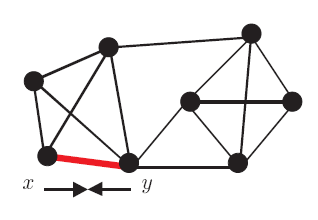
\includegraphics[width=\textwidth]{./images/contract-original-graph.png}
             \caption{Contrazione dell'arco $(x, y)$}
             \label{fig:original-graph}
     \end{subfigure}
   	\hfill
     \begin{subfigure}[b]{0.3\textwidth}
             \centering
             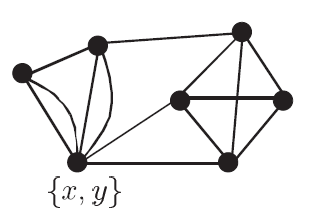
\includegraphics[width=\textwidth]{./images/contract-xy.png}
             \caption{Fusione in un vertice}
             \label{fig:contract-xy}
     \end{subfigure}
    \hfill
     \begin{subfigure}[b]{0.3\textwidth}
             \centering
             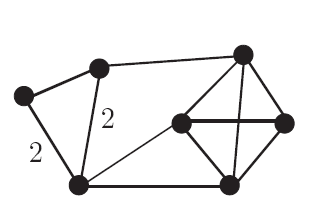
\includegraphics[width=\textwidth]{./images/after-contraction.png}
             \caption{Dopo la contrazione}
             \label{fig:after-contraction}
     \end{subfigure}
     \caption{Esempio di contrazione}
     \label{fig:contraction-example}
\end{figure}

\begin{listing}[!ht]
\begin{minted}{c++}
// Shared/AdjacencyMapGraph.h
TODO: describe the function in a paragraph, remove the comments
inline void AdjacencyMapGraph::contract(size_t contracted, size_t incorporator) {
    // delete every arc between contracted and incorporator.
    // One is the selected arc, the other ones would become self-loops, so we get rid of them.
    edge_count_map.erase({contracted, incorporator});
    adj_map[incorporator].erase(contracted);
    adj_map[contracted].erase(incorporator);

    // transfer every edge incident in contracted to incorporator.
    // Note that incorporator won't appear in contracted's adjacent nodes.
    for (const auto node : adj_map.at(contracted)) {
        // replace every arc (contracted, node) with a new (incorporator, node)
        adj_map[node].erase(contracted);
        adj_map[node].insert(incorporator);
        adj_map[incorporator].insert(node);

        const size_t n_multi_edge = edge_count_map.at({contracted, node});
        edge_count_map.erase({contracted, node});
        edge_count_map[{incorporator, node}] += n_multi_edge;
    }

    // delete contracted node
    adj_map.erase(contracted);
\end{minted}
\caption{Implementazione della contrazione del grafo.}
\label{listing:adjacency-map-graph-contract}
\end{listing}

\subsection{Analisi probabilistica}
\label{sub:karger-success-probability}

Per analizzare la probabilità che l'algoritmo di Karger non contragga il grafo proprio contraendo i due nodi del min-cut minimo ci baseremo su questa proprietà importante:

TODO: cambiare in proprietà
\begin{defn}
Sia $ G = (V, E) $ un multi-grafo con $ \lvert V \rvert = n$. Se $G$ ha un min-cut di cardinalità $t$, allora $\lvert E \rvert = \dfrac{t * n}{2}$
\end{defn}

Tale proprietà non verrà dimostrata (i dettagli della dimostrazione sono riportati in classe TODO).

A questo punto dobbiamo calcolare qual'è la probabilità di successo di un'esecuzione di full-contraction, ossia qual'è la probabilità che essa restituisca il taglio minimo del grafo.
Sia $E_{i}$ la probabilità che al passo i-esimo della full-contraction la scelta casuale non seleziona un arco del min-cut:

$$Pr(E_{1}) \geq 1-\dfrac{t}{t n/2}$$
$$Pr(E_{2} \mid E_{1}) \geq 1-\dfrac{t}{t (n-1)/2}$$
$$...$$
$$Pr(E_{i} \mid E_{1} \cup E_{2} \cup ... \cup E_{i-1}) \geq 1-\dfrac{t}{t (n-i+1)/2} = 1 - \dfrac{2}{n-i+1}$$

Ora, la probabilità che ad ogni iterazioni non scelgo un lato del min-cut è:

$$Pr(\bigcap_{i=1}^{n-2} E_{i}) \geq \prod_{i=1}^{n-2} (1 - \dfrac{2}{n-i+1}) = \dfrac{2}{n(n-1)} \geq \dfrac{2}{n^2}$$

\noindent Come possiamo notare questa probabilità è abbastanza bassa. Tuttavia se consideriamo ora la probabilità dell'evento complementare, ossia la probabilità che la nostra procedura di full-contraction non restituisca il taglio minimo del grafo e rieseguiamo la provedere per k volte, essendo ogni esecuzione di indipendente, otteniamo:
$$ Pr(\text{le k full-contraction non accumulano la taglia del min-cut}) \leq (1- \dfrac{2}{n^2})^k $$

\noindent scegliendo

$$ k = d * \dfrac{n^2}{2} * \log{n} $$

\noindent otteniamo
$$ Pr(\text{le k full-contraction non accumulano la taglia del min-cut}) \leq (\dfrac{1}{n^d}) $$

\noindent infatti

$$((1-\frac{2}{n^2})^{\frac{n^2}{2}} )^{\log{(n^d)}} \leq e^{-ln(n^d)} = \dfrac{1}{n^d}$$

\noindent che è proprio quello che volevamo per dimostrare che scelto k in questo modo, l'algoritmo di karger è corretto in alta probabilità.\\

\noindent $d$ è una costante che permette di abbassare la probabilità di fallimento dell'algoritmo di karger, infatti più $d$ sarà alto (di conseguenza più elevato sarà k), più sarà bassa la probabilità che l'algoritmo fallisca.


